\documentclass[12pt, letterpaper] {article}

\parindent=5mm
\usepackage[spanish]{babel}

\usepackage{amssymb}
\usepackage{amsmath} 
\usepackage{amsfonts}

\usepackage[numbers,sort&compress]{natbib}
\usepackage{graphicx}

\usepackage{url}
\usepackage{hyperref}

\usepackage[top=25mm, bottom=20mm, left=1.5cm, right=1.5cm]{geometry}
\setlength{\parskip}{2mm}
\setlength{\parindent}{1pt}

\usepackage{listings}

\usepackage{float}

\usepackage[utf8]{inputenc}
\usepackage{graphicx} 
\usepackage{subfigure} 

\usepackage{color}
\usepackage{multirow}

\definecolor{dkgreen}{rgb}{0,0.6,0}
\definecolor{gray}{rgb}{0.5,0.5,0.5}
\definecolor{mauve}{rgb}{0.58,0,0.82}

\usepackage{color}
\usepackage{listings}
\lstset{ %
  language=R,                     % the language of the code
  basicstyle=\footnotesize,       % the size of the fonts that are used for the code
  numbers=left,                   % where to put the line-numbers
  numberstyle=\tiny\color{gray},  % the style that is used for the line-numbers
  stepnumber=1,                   % the step between two line-numbers. If it's 1, each line
                                  % will be numbered
  numbersep=5pt,                  % how far the line-numbers are from the code
  backgroundcolor=\color{white},  % choose the background color. You must add \usepackage{color}
  showspaces=false,               % show spaces adding particular underscores
  showstringspaces=false,         % underline spaces within strings
  showtabs=false,                 % show tabs within strings adding particular underscores
  frame=single,                   % adds a frame around the code
  rulecolor=\color{black},        % if not set, the frame-color may be changed on line-breaks within not-black text (e.g. commens (green here))
  tabsize=2,                      % sets default tabsize to 2 spaces
  captionpos=b,                   % sets the caption-position to bottom
  breaklines=true,                % sets automatic line breaking
  breakatwhitespace=false,        % sets if automatic breaks should only happen at whitespace
  title=\lstname,                 % show the filename of files included with \lstinputlisting;
                                  % also try caption instead of title
  keywordstyle=\color{blue},      % keyword style
  commentstyle=\color{dkgreen},   % comment style
  stringstyle=\color{mauve},      % string literal style
  escapeinside={\%*}{*)},         % if you want to add a comment within your code
  morekeywords={*,...}            % if you want to add more keywords to the set
} 


\author{Dulce Esperanza Carrasco Castillo \\[0.9mm]}

\title{Estudio de la cinética de un adsorbente catiónico}


\date{\today}

\begin{document}


\twocolumn[
\begin{@twocolumnfalse}

\maketitle

\begin{center}\rule{0.9\textwidth}{0.1mm} \end{center}
\begin{abstract}

\normalsize 

Este trabajo describe la cinética de un adsorbente catiónico, se varía la fuerza de atracción del adsorbente (carga catiónica) de 0.02, 0.05 y 0.1 para los pasos 2, 5, 10, 15, 20, 30, 40, 50. Usando el software \texttt{Rproject} se grafican los resultados de número de partículas cargadas adsorbidas vs velocidad de adsorción (pasos), obteniendo que la fuerza de atracción 0.05 es la que obtuvo la mayor adsorción de partículas en menor cantidad de pasos, se realizó un ANOVA como prueba estadística para el paso diez donde los valores no son significativos, es decir, cualqueir fuerza de adsorción aplicada (0.02, 0.05, 0.1) es eficiente para la adsorción.\\ \\

Palabras clave: Adsorción, Cinética, Simulación, Interacción, Cargas.
\begin{center}\rule{0.9\textwidth}{0.1mm} \end{center}
\end{abstract}

\end{@twocolumnfalse} 
]

\section{Introducción}
Un adsorbente es un sólido que tiene la capacidad de retener en su superficie componentes presentes en un medio líquido o gaseoso, son comunmente usados para la eliminación de contaminantes en un medio. El adsorbente mayormente utilizado es el carbón activado el cual se puede sintetizar de cualquier compuesto orgánico llevado a pirólisis, también  los adsorbentes poliméricos son muy comunes. \par Existen tres tipos de adsorción, la química cuando el adsorbente forma enlaces con en adsorbato, la física que es regida por fuerzas de Van Der Waals y la adsorción por intercambio que es cuando los iones de cierta sustancia se atraen a la superficie del adsorbente por fuerzas electrostáticas.\par
Para determinar la eficiencia de un adsorbente es necesario analizar los aspectos cinéticos y termodinámicos\cite{art1}, el análisis cinético de un adsorbente nos indica la capacidad que tiene el adsorbente, es decir, la eficiencia en cuanto a rendimiento de adsorción.


\section{Antecedentes}
Se sabe que el uso de adsorbentes para eliminación de contaminantes en medios gaseosos y líquidos son muy estudiados y existe gran cantidad de artículos enfocados a estos, más en el área ambiental\cite{art2}. En el cso de carbón activado como adsorbente las investigaciones van enfocadas más a la fuente del carbón activado para su capacidad de adsorción, en cambio los adsrobentes de intercambio iónico también son de gran estudio ya que evitan las reacciones en el medio, por lo cual solo adsorben las partículas de cierta carga y se mantienen en la superficie del adsrobente.


\section{Herramientas}
La simulación se realizó en una laptop ASUS modelo X507M con un procesador Intel Celeron N4000. Haciendo uso del software \textit{R Project versión 3.5.3 (2019-03-11)}. Como base se usó la práctica 9 \cite{} de R paralelo: simulación y análisis de datos de la Dra. Shaeffer. 

\section{Experimentación}
Se crearon cien partículas cargadas aleatoriamente de -5 a 5, el algoritmo se modificó de tal forma de darle carga positiva al adsorbente de esta manera que las partículas con carga negativa fueran atraídas hacia el adsorbente. Se varió la fuerza de atracción de las partículas con valores de 0.02, 0.05 y 0.1, con 50 iteracciones y 3 réplicas para cada una, para medir la cinética se tomaron en cuenta los pasos con valores de 2, 5, 10, 15, 20, 30, 40 y 50, de manera de obtener la cantidad de partículas adsorbidas en cada paso, como prueba estadística se uso del ANOVA tomando los resultados del paso 10 para cada valor de fuerza.
%\begin{lstlisting}[language=R]

%\end{lstlisting}
 
\section{Resultados y discusión}
En la figura \ref{fig1} se pueden ver las partículas adsorbidas para cada valor de fuerza de atracción en el paso 10 de la cinética donde en la fuerza de atracción 0.02 es donde menos adsorbe.

\begin{figure}[h!]
\centering
\subfigure[Fuerza de atracción 0.05 ]{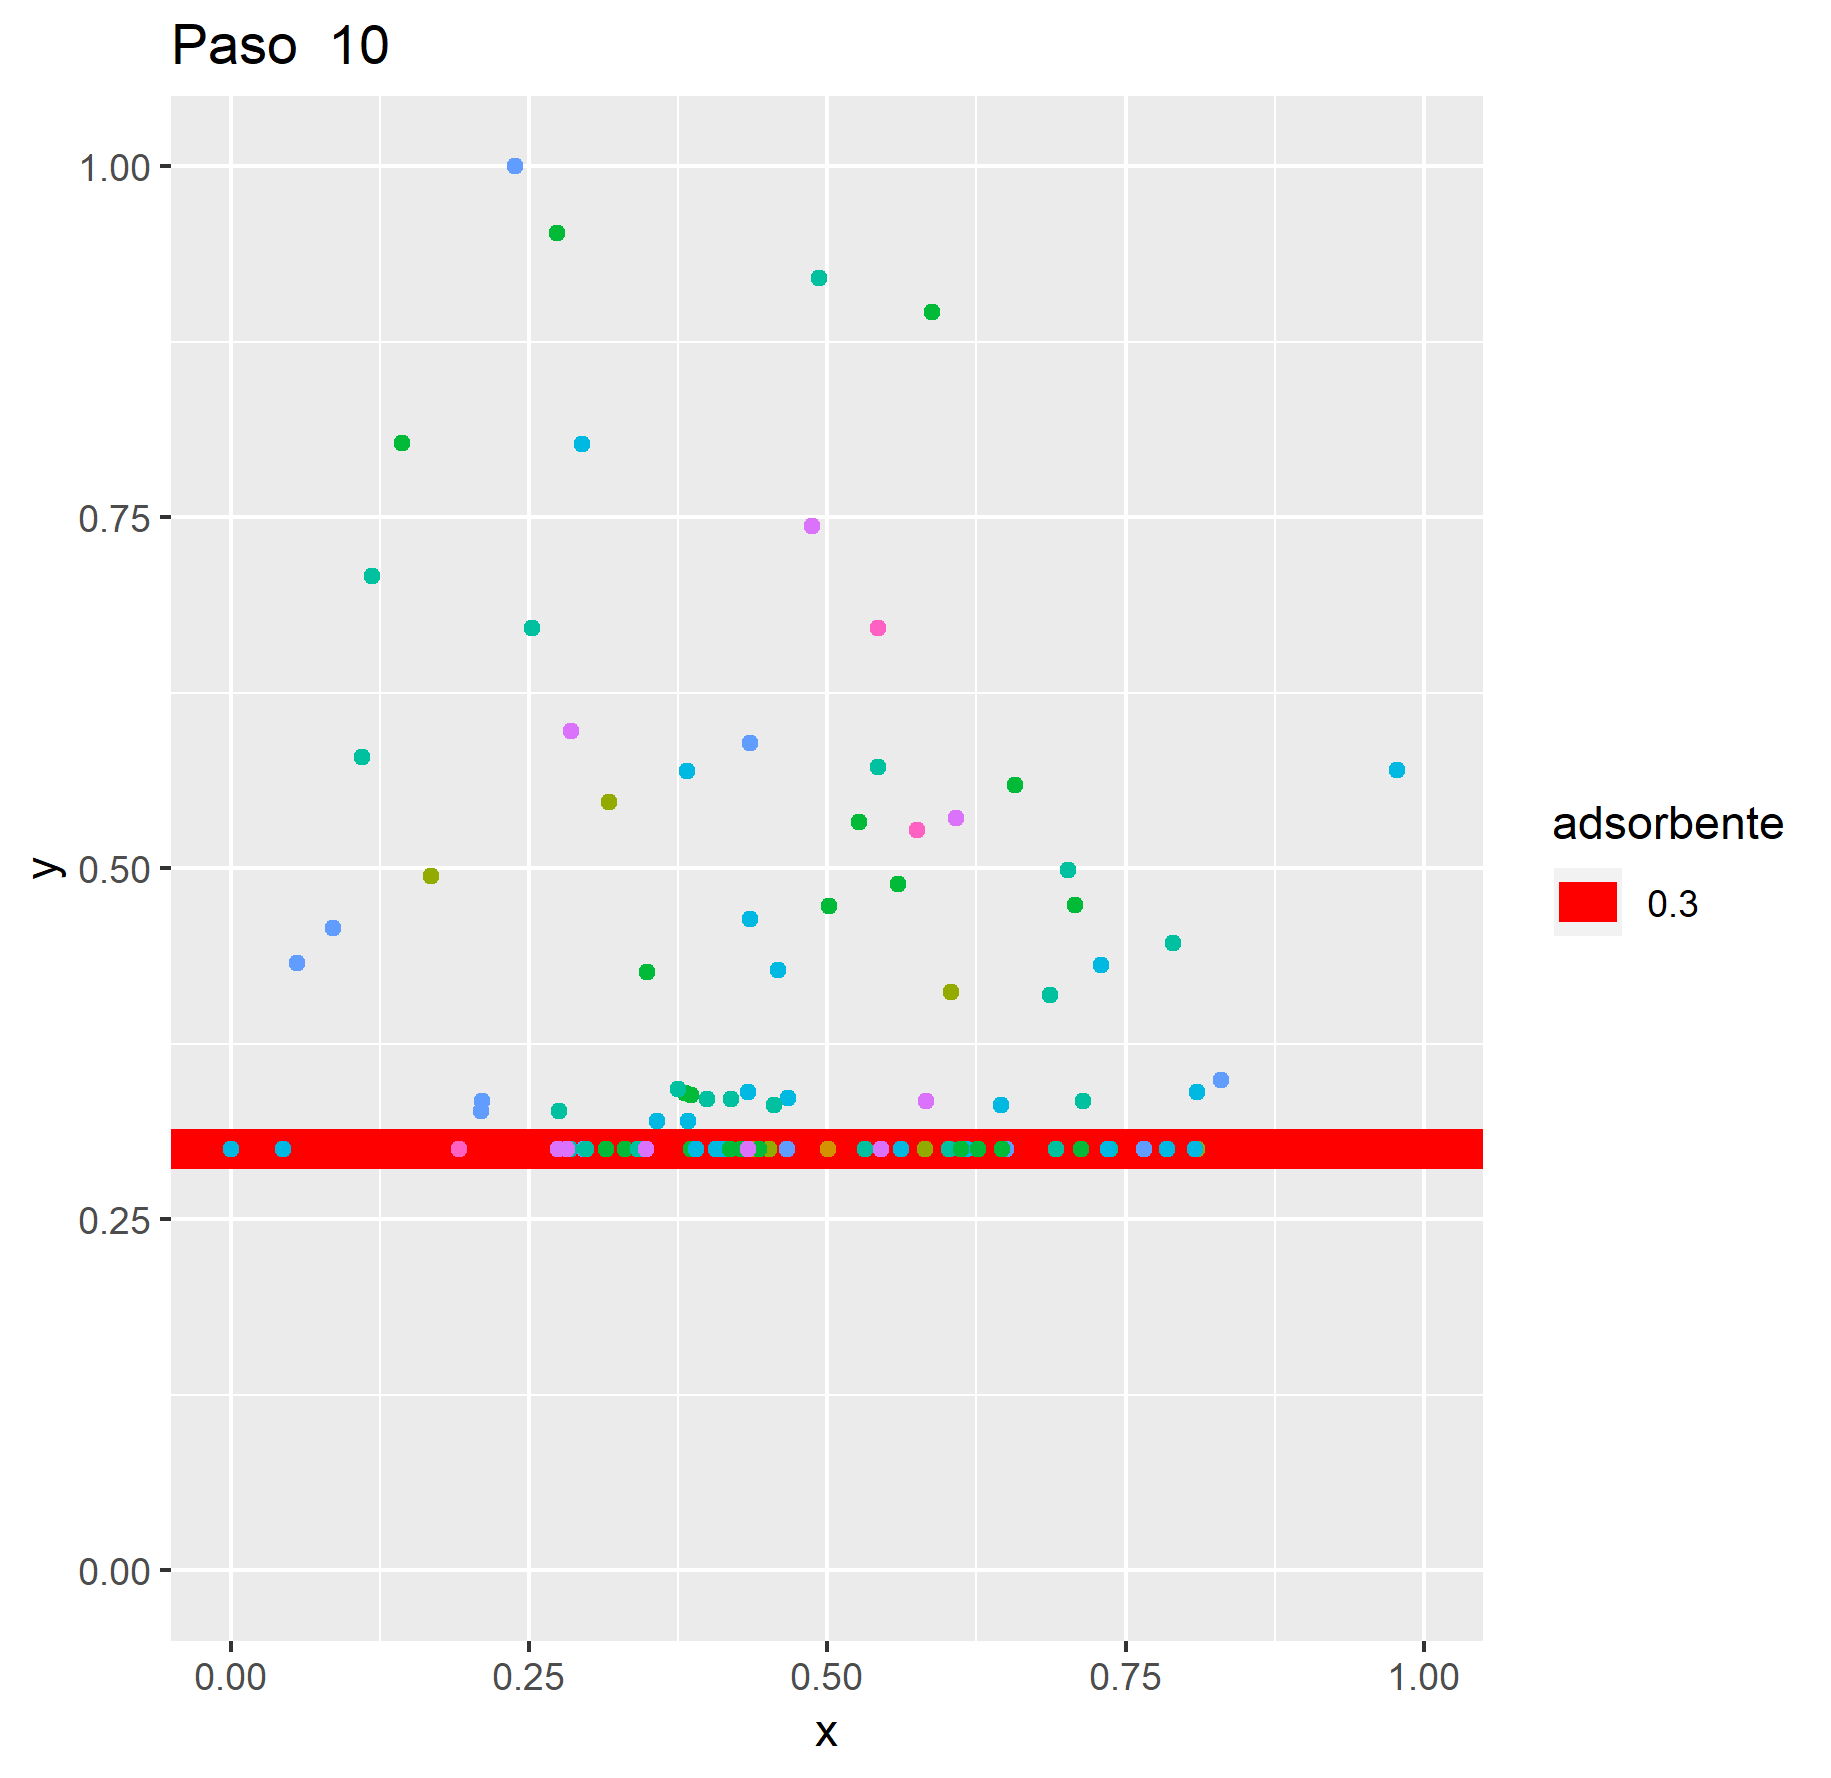
\includegraphics[width=60mm]{./f1p10.png}}
\subfigure[Fuerza de atracción 0.02]{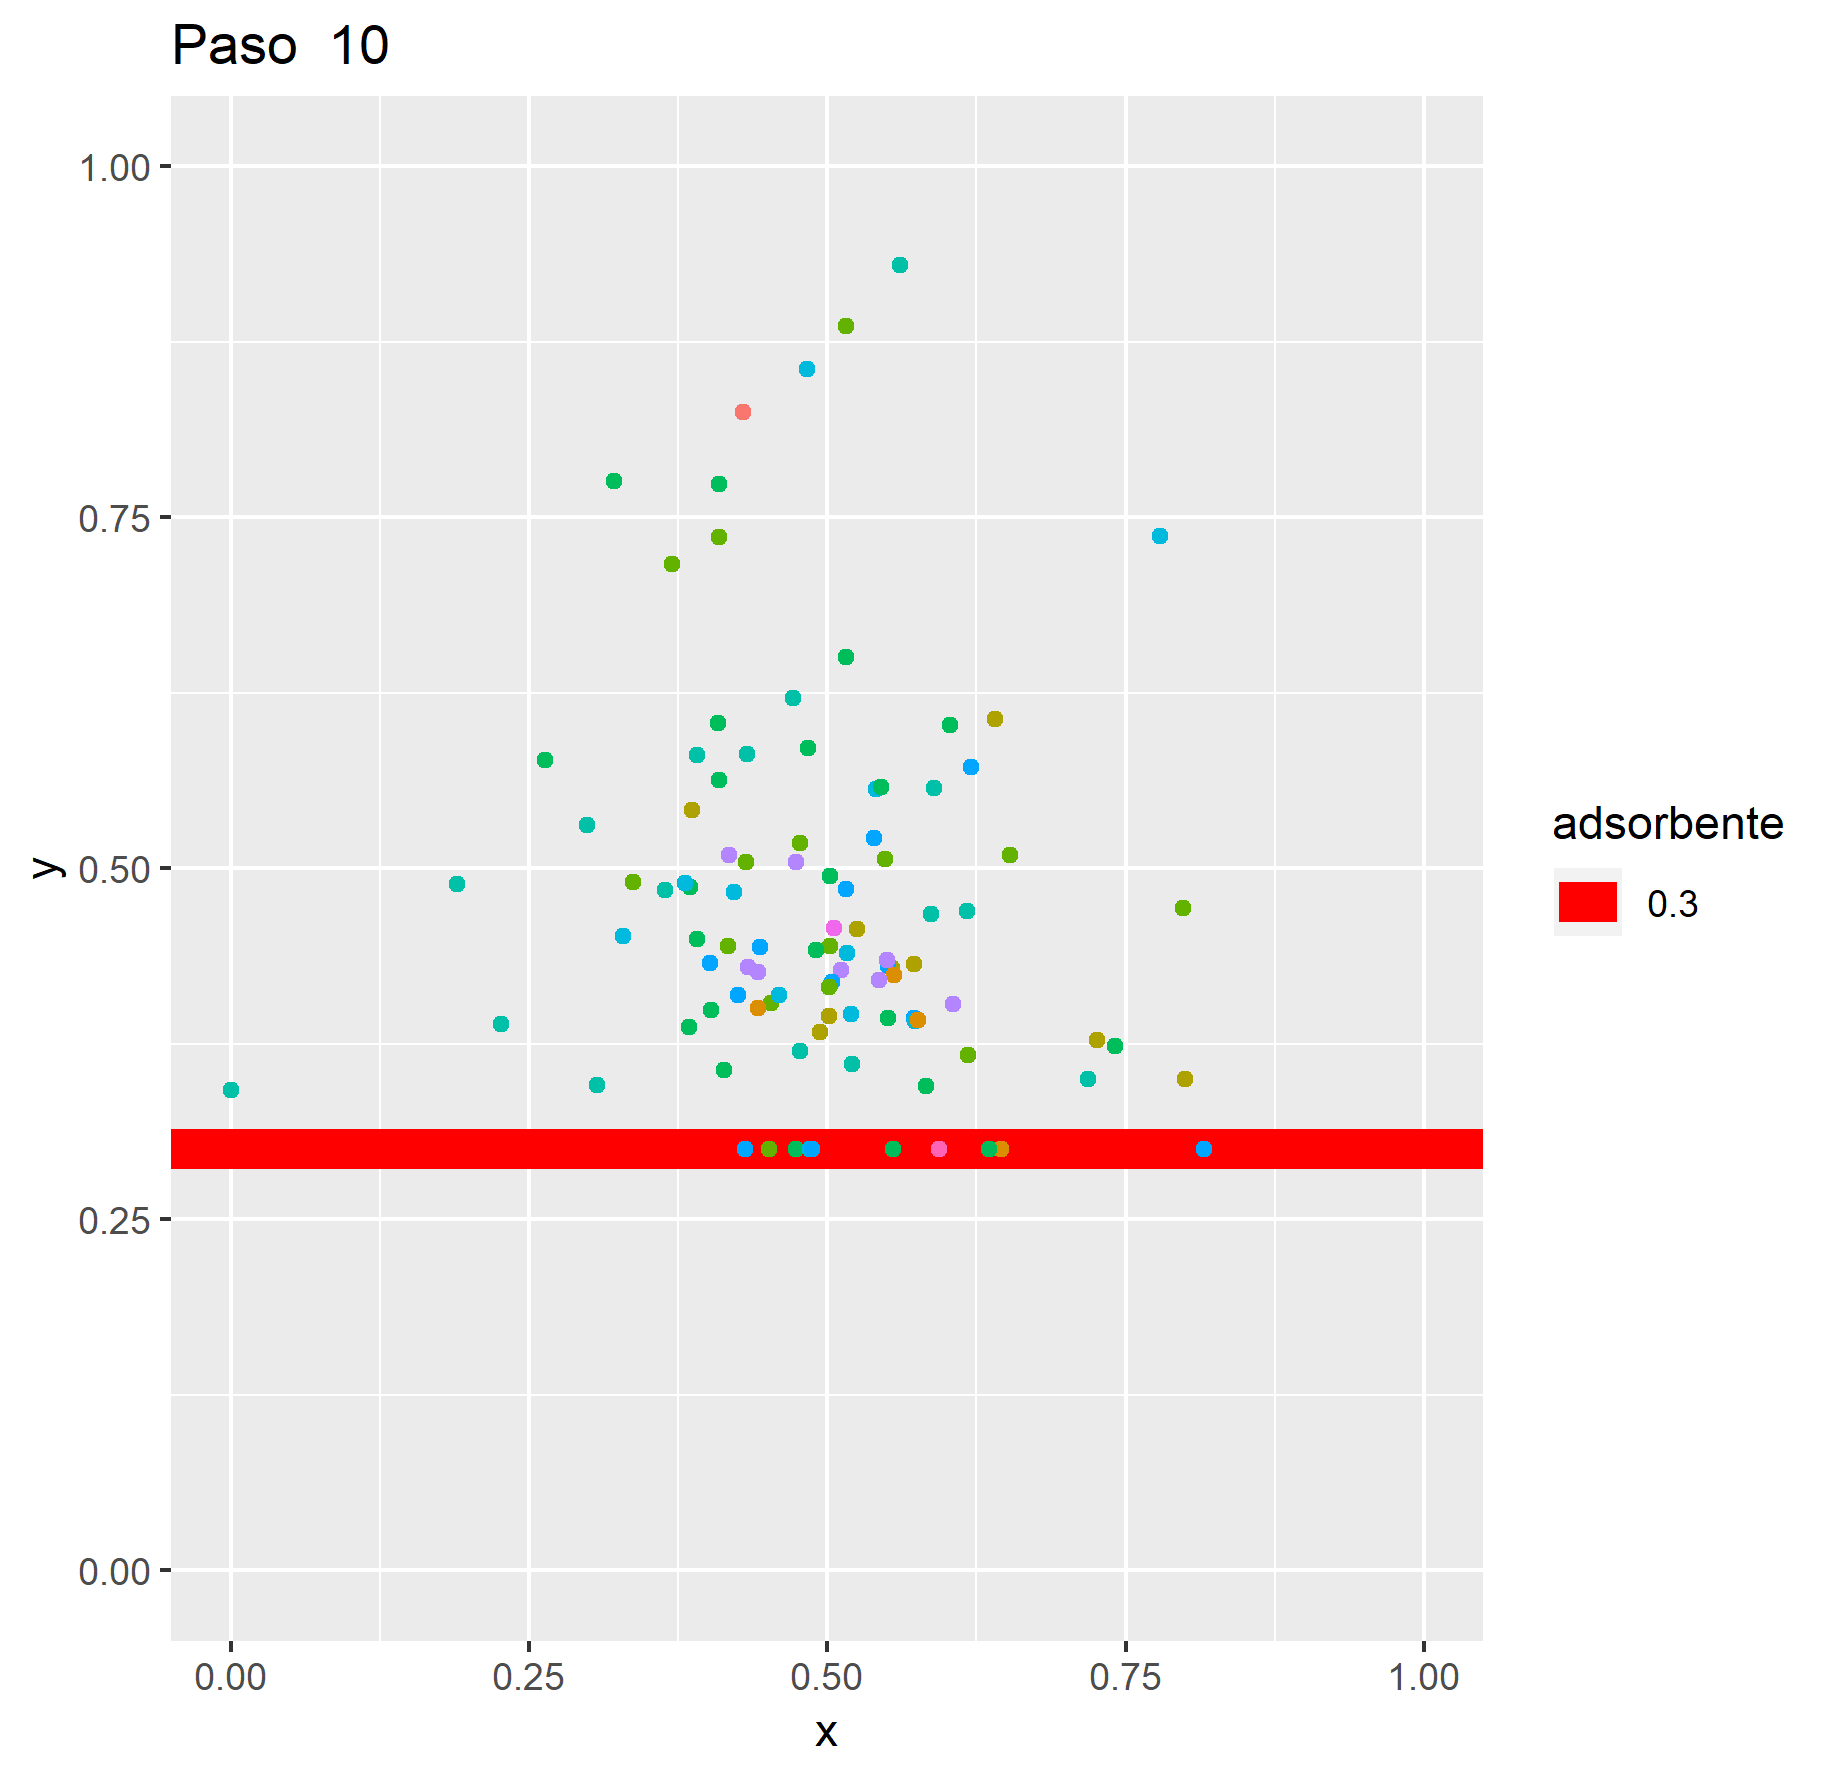
\includegraphics[width=60mm]{./f2p10.png}}
\subfigure[Fuerza de atracción 0.1 ]{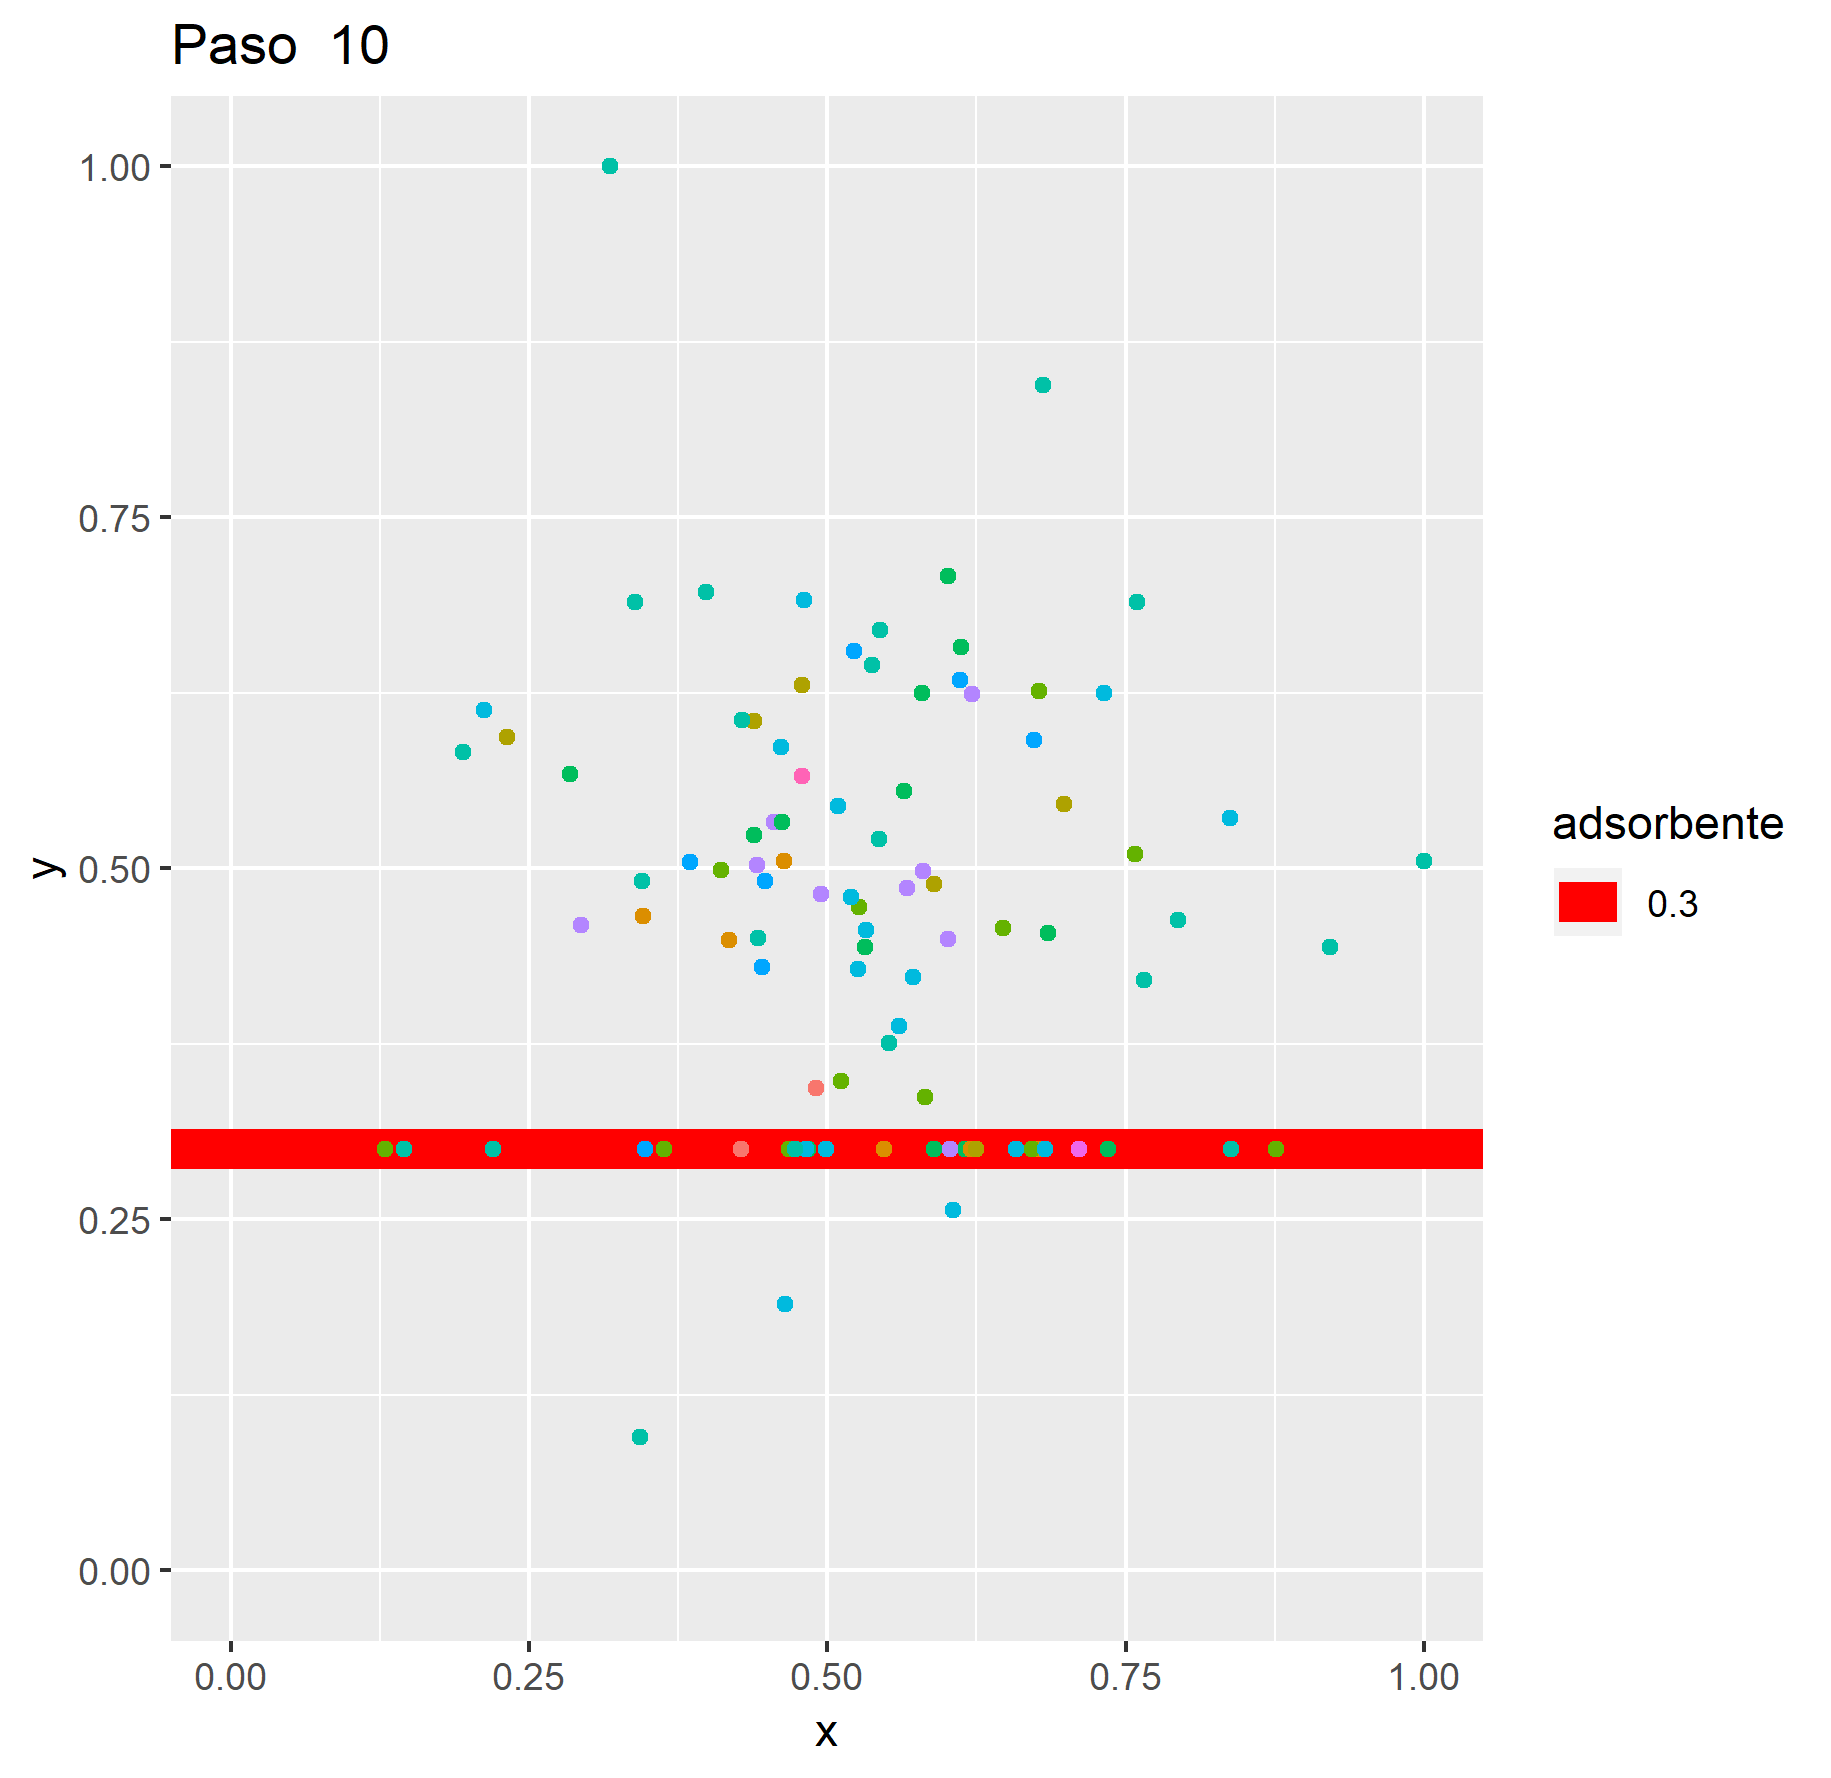
\includegraphics[width=60mm]{./f3p10.png}}
\caption{Partículas adsorbidas en el paso 10.} \label{fig1}
\end{figure}

Se puede observar en la figura \ref{fig2} que en donde hubo más partículas adsorbidas fue para la fuerza de atracción de 0.05, siguiendo de 0.02 y por último 0.1. También se puede observar que para la fuerza de atracción de 0.02 la adsroción de partículas incrementó considerablemente a partir del paso 15, en cambio para la fuerza de atracción de 0.05 fue una adsorción gradual.

\begin{figure*}[htb]
\centering
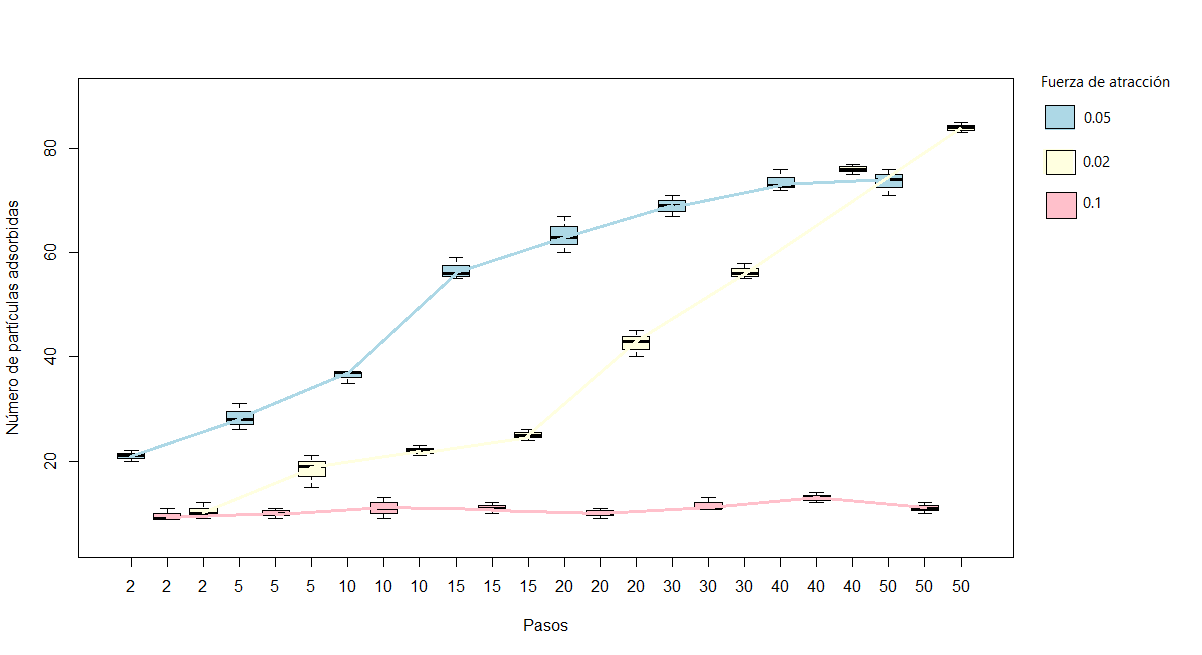
\includegraphics[width=1\textwidth]{Rplotcine.PNG}
\caption{Cinética del adsorbente catiónico. }
\label{fig2}
\end{figure*}
 Para la fuerza 0.1 se puede decir que la cantidad de partículas adsorbidas fueron casi las mismas en todos los pasos, de manera que lo que adsorbe al inicio es lo más que podrá adsorber a través del tiempo, esto es debido a la alta fuerza de atracción, es decir, a la alta carga catiónica del adsorbente, al concentrarse gran cantidad de cargas negativas cerca del adsorbente, esta misma fuerza en conjunto hace que se repelen entre ellas y no se adsorban, se podría pensar que la adsorción sería más eficiente con mayor cantidad de cargas positivas en el adsorbente, pero aquí se puede apreciar que no.

Como resultados del ANOVA se obtuvo un valor \textit{F} de 5.1432528497 y un valor \textit{P} de 0.00473561243 tomando un valor de significancia de 0.05, se puede decir que las fuerzas afectan significativamente al comportamiento del adsorbente.


\section{Conclusiones}
La cantidad de carga catiónica (fuerza de atracción) en un adsorbente catiónico determina si el adsorbente tendrá eficiencia, esto se puede saber a través de un análisis cinético del adsorbente, donde se sabe la capacidad de adsorción del mismo. En este caso se obtuvo que a una carga catiónica de 0.05 la adsorción de partículas fue gradual a través del tiempo, pero a cargas cationicas grandes el efecto de adsorción no es efectivo.

Conclusiones a futuro:\par
Se podría hacer más análisis cinéticos y variar las fuerzas con otros valores, incluir algún modelo matemático como base de la experimentación, incluso se podría tomar en cuenta la masa en el efecto de adsorción y la porosidad del adsorbente para ver de que manera afecta al rendimiento.
  
\section{Agradecimientos}
Se agradece al Dr. Martín Rosas por ayudar en la idea principal de este proyecto, también a Marcos Guajardo compañero de clase por asesorarme en el algoritmo de la simulación.


\bibliographystyle{plainnat}
\bibliography{biblioporta}




\end{document}